\documentclass[spec, och, labwork]{shiza}
% параметр - тип обучения - одно из значений:
%    spec     - специальность
%    bachelor - бакалавриат (по умолчанию)
%    master   - магистратура
% параметр - форма обучения - одно из значений:
%    och   - очное (по умолчанию)
%    zaoch - заочное
% параметр - тип работы - одно из значений:
%    referat    - реферат
%    coursework - курсовая работа (по умолчанию)
%    diploma    - дипломная работа
%    pract      - отчет по практике
% параметр - включение шрифта
%    times    - включение шрифта Times New Roman (если установлен)
%               по умолчанию выключен
\usepackage{subfigure}
\usepackage{tikz,pgfplots}
\pgfplotsset{compat=1.5}
\usepackage{float}

%\usepackage{titlesec}
\setcounter{secnumdepth}{4}
%\titleformat{\paragraph}
%{\normalfont\normalsize}{\theparagraph}{1em}{}
%\titlespacing*{\paragraph}
%{35.5pt}{3.25ex plus 1ex minus .2ex}{1.5ex plus .2ex}

\titleformat{\paragraph}[block]
{\hspace{1.25cm}\normalfont}
{\theparagraph}{1ex}{}
\titlespacing{\paragraph}
{0cm}{2ex plus 1ex minus .2ex}{.4ex plus.2ex}

% --------------------------------------------------------------------------%


\usepackage[T2A]{fontenc}
\usepackage[utf8]{inputenc}
\usepackage{graphicx}
\graphicspath{ {./images/} }
\usepackage{tempora}

\usepackage[sort,compress]{cite}
\usepackage{amsmath}
\usepackage{amssymb}
\usepackage{amsthm}
\usepackage{fancyvrb}
\usepackage{listings}
\usepackage{listingsutf8}
\usepackage{longtable}
\usepackage{array}
\usepackage[english,russian]{babel}

% \usepackage[colorlinks=true]{hyperref}
\usepackage{url}

\usepackage{underscore}
\usepackage{setspace}
\usepackage{indentfirst} 
\usepackage{mathtools}
\usepackage{amsfonts}
\usepackage{enumitem}
\usepackage{tikz}
\usepackage{minted}

\newcommand{\eqdef}{\stackrel {\rm def}{=}}
\newcommand{\specialcell}[2][c]{%
\begin{tabular}[#1]{@{}c@{}}#2\end{tabular}}

\renewcommand\theFancyVerbLine{\small\arabic{FancyVerbLine}}

\newtheorem{lem}{Лемма}

\begin{document}

% Кафедра (в родительном падеже)
\chair{}

% Тема работы
\title{Идеалы полугрупп}

% Курс
\course{3}

% Группа
\group{331}

% Факультет (в родительном падеже) (по умолчанию "факультета КНиИТ")
\department{факультета КНиИТ}

% Специальность/направление код - наименование
%\napravlenie{09.03.04 "--- Программная инженерия}
%\napravlenie{010500 "--- Математическое обеспечение и администрирование информационных систем}
%\napravlenie{230100 "--- Информатика и вычислительная техника}
%\napravlenie{231000 "--- Программная инженерия}
\napravlenie{100501 "--- Компьютерная безопасность}

% Для студентки. Для работы студента следующая команда не нужна.
% \studenttitle{Студентки}

% Фамилия, имя, отчество в родительном падеже
\author{Окунькова Сергея Викторовича}

% Заведующий кафедрой
% \chtitle{} % степень, звание
% \chname{}

%Научный руководитель (для реферата преподаватель проверяющий работу)
\satitle{аспирант} %должность, степень, звание
\saname{В. Н. Кутин}

% Руководитель практики от организации (только для практики,
% для остальных типов работ не используется)
% \patitle{к.ф.-м.н.}
% \paname{С.~В.~Миронов}

% Семестр (только для практики, для остальных
% типов работ не используется)
%\term{8}

% Наименование практики (только для практики, для остальных
% типов работ не используется)
%\practtype{преддипломная}

% Продолжительность практики (количество недель) (только для практики,
% для остальных типов работ не используется)
%\duration{4}

% Даты начала и окончания практики (только для практики, для остальных
% типов работ не используется)
%\practStart{30.04.2019}
%\practFinish{27.05.2019}

% Год выполнения отчета
\date{2022}

\maketitle

% Включение нумерации рисунков, формул и таблиц по разделам
% (по умолчанию - нумерация сквозная)
% (допускается оба вида нумерации)
% \secNumbering

%-------------------------------------------------------------------------------------------
\tableofcontents

\section{Постановка задачи}

  \textbf{Цель работы:} изучение строения полугрупп с помощью отношений Грина.
  
  Порядок выполнения работы:
    \begin{enumerate}
        \item Рассмотреть понятия идеалов полугруппы. Разработать алгоритмы построения идеалов полугруппы по таблице Кэли.
        \item Рассмотреть понятия и свойства отношений Грина на полугруппах.
        \item Разработать алгоритмы вычисления отношений Грина и построения <<egg-box>>-картины конечной полугруппы.
    \end{enumerate}

\section{Теоретические сведения по рассмотренным темам с их обоснованием}

  Пусть $S$ -- произвольная полугруппа.\\
  \textbf{Определение 1.} Полугруппа – это алгебра S = (S, ·) с одной ассоциативной бинарной
    операцией $\cdot$, т.е. выполняется
      \begin{center}
        $(x \cdot y) \cdot z = x \cdot (y \cdot z)$
      \end{center}
    для любых $x,y,z \in S$.
    
    \textbf{Определение 2.} Непустое подмножество $I \subset S$ называется правым (левым) идеалом полугруппы $S$,
    если для любых $x \in I$, $y \in S$ выполняется условие: $xy \in I$ ($yx \in I$), т.е. $I \cdot S \subset I$ ($S \cdot I \subset I$).
    Если $I$ -- одновременно левый и правый идеал полугруппы $S$, то $I$ называется двусторонним идеалом (или просто идеалом) полугруппы
    $S$. Ясно, что в коммутативной полугруппе $S$ все эти определения совпадают.

    \textbf{Лемма 1.} Множество всех идеалов $Id S$  (соответственно, левых идеалов $LId S$  или правых идеалов $RId S$) любой
    полугруппы $S$ является системой замыкания. Пусть $X$ -- подмножество полугруппы $S$. Тогда наименьший правый идеал 
    полугруппы $S$, содержащий подмножество $X$, равен $(X] = XS^1 = X \cup XS$, наименьший левый идеал полугруппы $S$, содержащий
    подмножество $X$, равен $[X) = S^1X = X \cup SX$  и наименьший идеал полугруппы $S$, содержащий подмножество $X$, равен 
    $[X] = S^1XS^1 = X \cup XS \cup SX \cup SXS$.
    
    В частности, любой элемент $a \in S$ определяет наименьшие правый, левый и двусторонний идеалы: $(a] = aS^1$, $[a) = S^1a$ и
    $[a] = S^1aS^1$, которые называются главными (соответственно, правыми, левыми и двусторонними) идеалами.
    Минимальные относительно теоретико-множественного включения идеалы (левые или правые идеалы) называются минимальными идеалами
    (минимальными левыми или правыми идеалами).
    
    \textbf{Лемма 2.} Если полугруппа имеет минимальный идеал, то он является ее наименьшим идеалом и называется ядром полугруппы.

    \underline{Пример:} В полугруппе натуральных чисел с операцией сложения $\textbf{N} = (\textbf{N}, +)$ главные идеалы 
    $(n] = {n, n + 1, n + 2, \dots}$ образуют бесконечную последовательность с пустым пересечением.

    \begin{center}
      Отображения $f: a \mapsto [a]$, $f_r: a \mapsto (a]$, $f_l: a \mapsto [a)$, $a \in S$ определяют ядра $\mathfrak{J} = ker f$,
      $\mathfrak{R} = ker f_r$, $\mathfrak{L} = ker f_l$ по формулам:

      $(a, b) \in \mathfrak{J} \Longleftrightarrow [a] = [b]$,

      $(a, b) \in \mathfrak{R} \Longleftrightarrow (a] = (b]$,

      $(a, b) \in \mathfrak{L} \Longleftrightarrow [a) = [b)$.
    \end{center}

    Все эти отношения, а также отношения $\mathfrak{D}  = \mathfrak{R} \vee \mathfrak{L}$, $\mathfrak{H}  = \mathfrak{R} \cap \mathfrak{L}$
    являются эквивалентностями на множестве $S$, которые называются \textbf{отношениями Грина} полугруппы $S$. Классы этих эквивалентностей,
    порожденные элементом $a \in S$, обозначаются $J_a$, $R_a$, $L_a$, $D_a$ и $H_a$, соответственно.
  
    \textbf{Лемма 3.} Отношения Грина полугруппы $S$ удовлетворяют следующим свойствам:

    \begin{enumerate}
      \item эквивалентность $\mathfrak{R}$ регулярна слева и эквивалентность $\mathfrak{L}$ регулярна справа, т.е.
      $(a, b) \in \mathfrak{R} \Rightarrow (xa, xb) \in \mathfrak{R}$ и $(a, b) \in \mathfrak{L} \Rightarrow (ax, bx) \in \mathfrak{L}$ 
      для любых $x \in S$;
      \item эквивалентности $\mathfrak{R}$, $\mathfrak{L}$ коммутируют;
      \item $\mathfrak{D} = \mathfrak{R} \cdot \mathfrak{L} = \mathfrak{L} \cdot \mathfrak{R}$;
      \item если полугруппа $S$ конечна, то $\mathfrak{D} = \mathfrak{J}$;
      \item любой класс $\mathfrak{D}$ эквивалентности $\mathfrak{D}$ можно изобразить с помощью следующей <<egg-box>>-диаграммы,
      клетки которой являются классами эквивалентности $\mathfrak{H}$, лежащими в $\mathfrak{D}$.
    \end{enumerate}


      \begin{figure}[H]
        \centering
        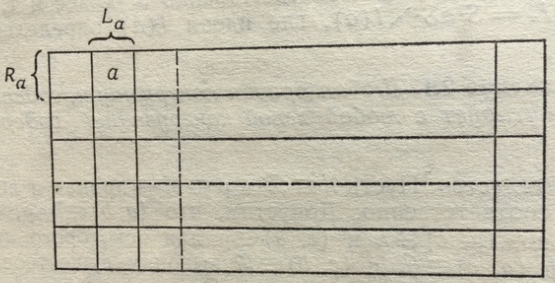
\includegraphics[width=0.8\textwidth]{pic/egg-box.png}
        \caption{<<egg-box>>-диаграмма}
      \end{figure}

      \section{Результаты работы}
      \subsection{Алгоритм 1 -- Построение правых идеалов полугруппы по таблице Кэли}
  
      \textit{Вход}: Конечная полугруппа $S$ с таблицей Кэли $A = (a_{ij})$ размерности $n \times n$ и элементом $x \in S$.
  
      \textit{Выход}: Правый идеал $Id_R$ полугруппы $S$, порожденный элементом $x \in S$.
      
      \underline{Шаг 1.} Инициализировать пустое множество $Id_R = \{\}$. Получить индекс $index$ заданного элемента $x \in semigroup$.
      Стоит отметить, что полугруппа $S$ представлена в виде списка $semigroup$.
      
      \underline{Шаг 2.} Пройти по элементам строки таблицы Кэли $a[index][i]$, где $0 \leq i < n$. Если элемент $a[index][i]$ ($0 \leq i < n$) еще не содержится
      в множестве $Id_R$, то он добавляется в это множество.
      
      \underline{Шаг 3.} Вернуть множество $Id_R$ в качестве ответа.
      
        Оценка сложности алгоритма равна $O(nlog n)$.
  
        \subsection{Алгоритм 2 -- Построение левых идеалов полугруппы по таблице Кэли}
  
      \textit{Вход}: Конечная полугруппа $S$ с таблицей Кэли $A = (a_{ij})$ размерности $n \times n$ и элементом $x \in S$.
  
      \textit{Выход}: Левый идеал $Id_L$ полугруппы $S$, порожденный элементом $x \in S$.
      
      \underline{Шаг 1.} Инициализировать пустое множество $Id_L = \{\}$. Получить индекс $index$ заданного элемента $x \in semigroup$.
      Стоит отметить, что полугруппа $S$ представлена в виде списка $semigroup$.
      
      \underline{Шаг 2.} Пройти по элементам столбца таблицы Кэли $a[i][index]$, где $0 \leq i < n$. Если элемент $a[i][index]$ ($0 \leq i < n$)
      еще не содержится в множестве $Id_L$, то он добавляется в это множество.
      
      \underline{Шаг 3.} Вернуть множество $Id_L$ в качестве ответа.
      
        Оценка сложности алгоритма равна $O(nlog n)$.
  
        \subsection{Алгоритм 3 -- Построение двусторонних идеалов полугруппы по таблице Кэли}
  
      \textit{Вход}: Конечная полугруппа $S$ с таблицей Кэли $A = (a_{ij})$ размерности $n \times n$ и элементом $x \in S$.
  
      \textit{Выход}: Двусторонний идеал $Id$ полугруппы $S$, порожденный элементом $x \in S$.
      
      \underline{Шаг 1.} Вызвать алгоитм 1 и 2 для таблицей Кэли $A = (a_{ij})$ и элемента $x$, в результате которых получаем
      множества $RI$ и $LI$.
      
      \underline{Шаг 2.} Вернуть множество $Id$ в качестве ответа, которое будет представлять из себя объединение множеств $RI$ и $LI$.
      
        Оценка сложности алгоритма равна $O(nlog n)$.
  
  
      \subsection{Алгоритм 4 -- Построение отношения Грина по таблице Кэли}
  
      \textit{Вход}: Конечная полугруппа $S$ с таблицей Кэли $A = (a_{ij})$ размерности $n \times n$ и элементом $x \in S$.
  
      \textit{Выход}: Матрица $D = (d_{ij})$ отношения Грина.
      
      \underline{Шаг 1.} Используя алгоритм 1, построим список $right\_ideals$, элементы которого будут правые идеалы $Id_{R_0}, \dots, Id_{R_{n-1}}$ порожденные
      элементами $x_i \in S$, где $0 \leq i < n$. Аналогично, используя алгоритм 2, построим список $left\_ideals$, элементы которого будут правые идеалы
      $Id_{L_0}, \dots, Id_{L_{n-1}}$ порожденные элементами $x_i \in S$, где $0 \leq i < n$.
      
      \underline{Шаг 2.}  Построим матрицу $R = (r_{ij})$. Пусть $i = 0$ и $el = right\_ideals[i]$. Необходимо пройти по всем элементам $Id_{R_j}$ ($0 \leq j < n$)
      списка $right\_ideals$, чтобы выполнить следующее условие: если $el = Id_{R_j}$ ($0 \leq j < n$), то $d[i][j] = 1$, в противном случае -- $d[i][j] = 0$.
      После того, как $j = n$, необходимо присвоить $i = i + 1$ и осуществить проход по элементам $Id_{R_0}, \dots, Id_{R_{n-1}}$ списка $right\_ideals$ повторно.
      В итоге получим матрицу $R$.
      
      \underline{Шаг 3.} Аналогично построим матрицу $L = (l_{ij})$, только уже используя список $left\_ideals$. В итоге получаем матрицу $L$.
  
      \underline{Шаг 4.} Построим матрицу $D = R + L$, т.е. $d[i][j] = r[i][j] + l[i][j]$, где $0 \leq i, j < n$. Учитывая, что если $r[i][j] = l[i][j] = 1$,
      то $d[i][j] = 1$.
  
      \underline{Шаг 5.} Вернуть в качестве ответа матрицу $D$, так как она, в свою очередь, является представлением отношения Грина.
      
        Оценка сложности алгоритма равна $O(n^2)$.
  
  
      \subsection{Алгоритм 5 -- Построение <<egg-box>>-диаграммы}
  
        \textit{Вход}: Конечная полугруппа $S$ с таблицей Кэли $A = (a_{ij})$ размерности $n \times n$ и элементом $x \in S$.
  
        \textit{Выход}: <<egg-box>>-картина конечной полугруппы $S$.
        
        \underline{Шаг 1.} Запустив последовательно алгоритмы 1, 2 и 4, получим отношение Грина, выраженного матрицей $D = (d_{ij})$ (обстрактно его можно представть как граф).
  
        \underline{Шаг 2.} Необходимо в матрице $D$ найти все компоненты сильной связности. Для этого можно использовать алгоритм конденсации графа или алгоритм Тарьяна. В результате получаем
        список $egg\_box\_list$, состоящего из элементов $x_i \in S$, ($0 \leq i < n$) и элемента 1, так как <<egg-box>>-картина строится по полугруппе
        с внешне присоединенной единицей $S^1 = S \cup \{1\}$.
  
        Оценка сложности равна оценке сложность алгоритма 6, т.е. $O(n + n) = O(n)$
  
        \subsection{Алгоритм 6 -- Построение полугруппы по порождающему множеству и определяющим соотношениям}
  
        \textit{Вход}: Конечное множество символов $A$ мощности $n$ и конечное множество $R$ определяющих соотношений мощности $m$.
  
        \textit{Выход}: Полугруппа $\langle A | R \rangle$.
  
        \underline{Шаг 1.} Необходимо инициализировать список $semigroup = []$, в который будут добавлены все элементы $a \in A$.
        
        \underline{Шаг 2.} Инициализировать список $elements_{new} = []$.
  
        \underline{Шаг 3.} Далее возьмем элемент $x \in semigroup$ и <<умножим>> его на $y \in semigroup$, получая новое слово
        $z = xy$. Далее полученное слово необходимо обработать, используя соотношение $r \in R$. После всех преобразований получим слово $z^{'}$.
        Добавим полученное слово в список $elements_{new}$.
  
        \underline{Шаг 4.} Инициализировать список $semigroup_{check} = semigroup$ (т.е. делается копия списка $semigroup$). Далее добавляем
        элементы $z^{'} \in elements_{new}$ в список $semigroup$, если их еще нет в списке $semigroup$. 
  
        \underline{Шаг 5.} Если после после шага 4 переменная $semigroup = semigroup_{check}$, то завершить алгоритм, иначе вернуться к шагу 2.
  
        Оценка сложности алгоритма примерно равна $O((n - 1) \cdot n^n \cdot m)$, так как трудно оценить из-за наличия бесконеного цикла в реализации
        данного алгоритма.

        \subsection{Коды программ, реализующей рассмотренные алгоритмы}

        \inputminted[fontsize=\small]{python}{../code/lab5.py}

      \newpage
      
      \subsection{Результаты тестирования программ}
      
      \begin{figure}[H]
        \centering      %размер рисунка       здесь находится название файла рисунка, без указания формата
        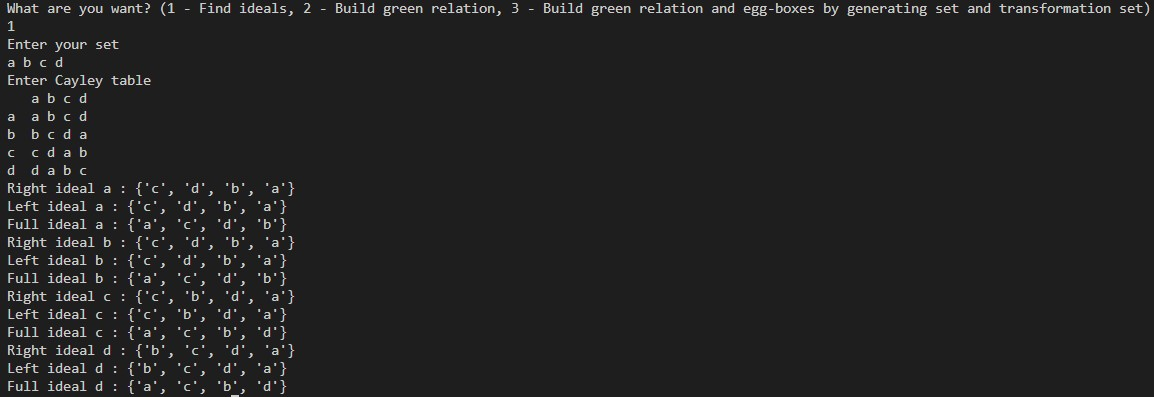
\includegraphics[width=1.\textwidth]{pic/1}
        \caption{Тест алгоритма поиска идеалов}
        \label{fig:image1}
    \end{figure}

    \begin{figure}[H]
        \centering      %размер рисунка       здесь находится название файла рисунка, без указания формата
        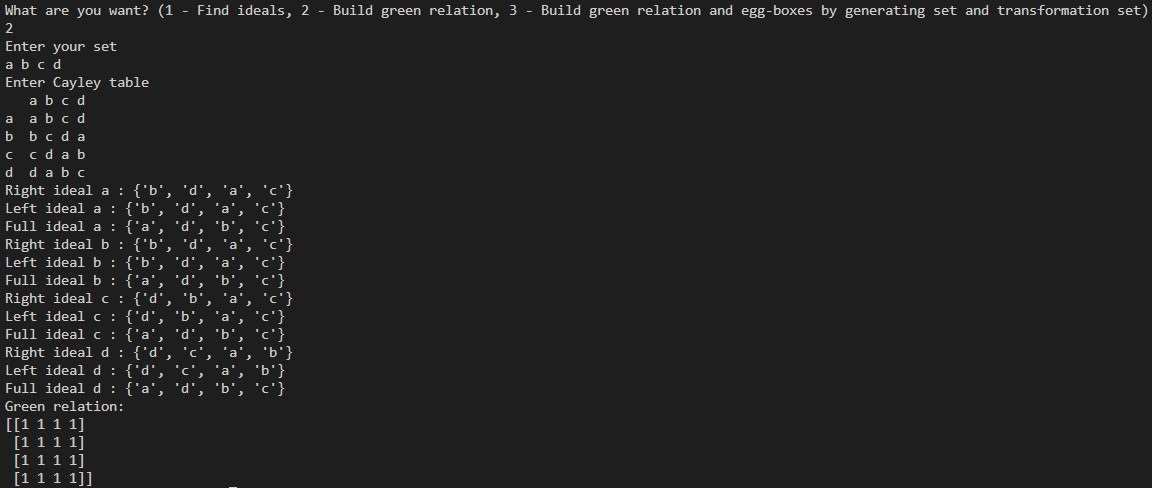
\includegraphics[width=1.\textwidth]{pic/2}
        \caption{Тест алгоритма построения отношения Грина}
        \label{fig:image1}
    \end{figure}

    \begin{figure}[H]
        \centering      %размер рисунка       здесь находится название файла рисунка, без указания формата
        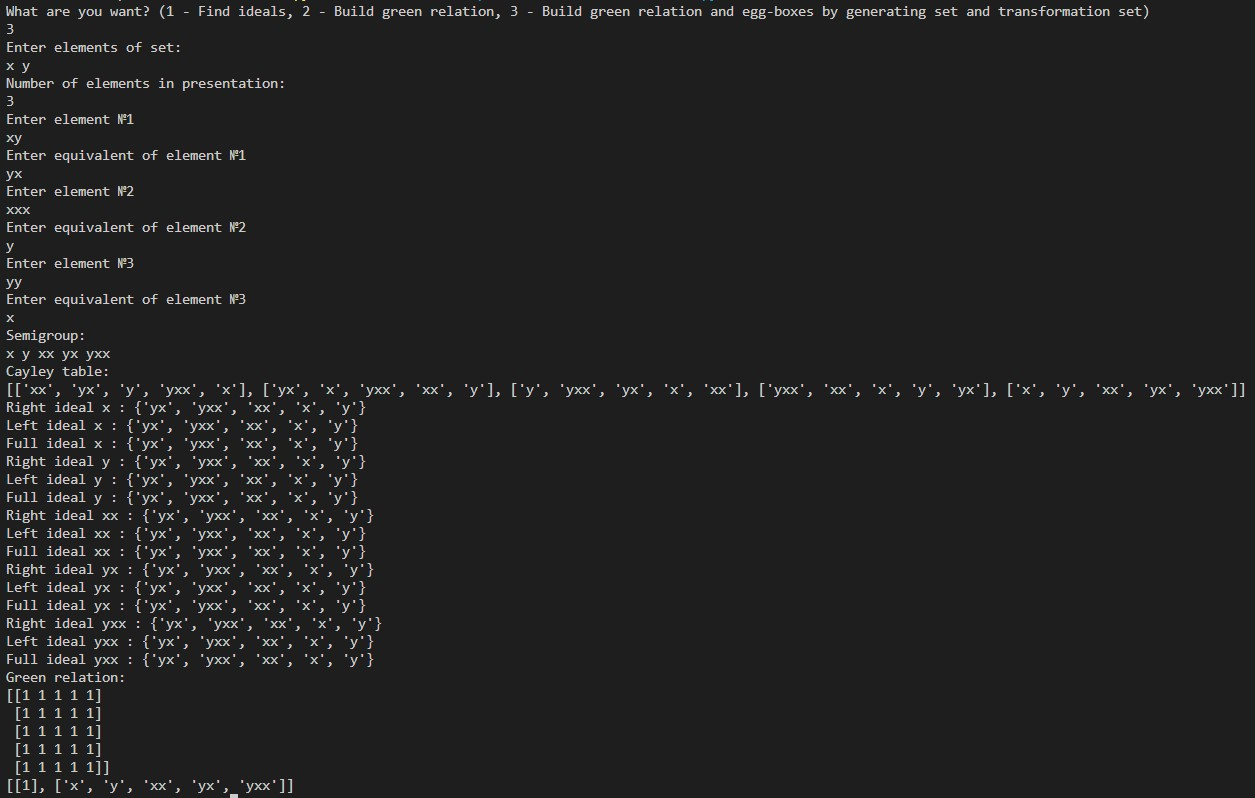
\includegraphics[width=1.\textwidth]{pic/3}
        \caption{Тест алгоритма построения отношения Грина и egg-box-ов по порождающему
        множеству и определяющим соотношениям}
        \label{fig:image1}
    \end{figure}

    \subsection{Ответы на задачи}
      \textbf{Задание 1.} Найдите подполугруппу $\langle x \rangle$, правый $(x]$, левый $[x)$ и двусторонний $[x]$ идеалы
      полугруппы $S$, порожденные элементом $x$, и определите порядок элемента x для каждого элемента полугруппы, на
      которой бинарная операция задана следующей таблицей Кэли:
        \begin{table}[H]
            \centering
            \begin{tabular}{|l|l|l|l|l|}
            \hline
            $\cdot$ & a & b & c & d \\ \hline
            a & a & b & c & d \\ \hline
            b & b & c & d & a \\ \hline
            c & c & d & a & b \\ \hline
            d & d & a & b & c \\ \hline
        \end{tabular}
        \end{table}

    \begin{enumerate}
      \item Нахождение подполугруппы:
    
      Подполугруппа строится по порождающему ее множеству. Допустим у нас есть подмножество $X \subset S$, где $X = \{ a\}$. 
      Тогда построим подполгруппу:
  
      Элемент $a$ подмножества $X$ определен в первой строчке таблицы Кэли. Поэтому мы должны пройти по элементам, находящихся в первой
      строке. Если еще такого элемента нет в подмножестве $X$, то он добавляется в данное подмножество. Т.е. пройдя по первой строке в
      данном случае получается подмножество $X = \{a, b, c, d\}$. Далее необходимо пройтись по строчкам, в котором определены новые элементы
      подмножества $X$ (т.е. $b, c, d$). Рассмотрим элемент $b$ и, пройдясь по второй строчке, видно, что новых элементов в подмножество $X$
      не добавилось. Значит, мы получили подполугруппу $\langle X \rangle = \{a, b, c, d\}$.  

      Аналогично строится подполугруппа для $b,c,d$ полугруппы $S$:

      Пусть $X \subset S$, где $X = \{b\}$. Тогда $\langle X \rangle = \{a, b, c, d\}$.

      Пусть $X \subset S$, где $X = \{c\}$. Тогда $\langle X \rangle = \{a, b, c, d\}$.

      Пусть $X \subset S$, где $X = \{d\}$. Тогда $\langle X \rangle = \{a, b, c, d\}$.
      
      \item Нахождение идеалов:
      
      Используя таблицу Кэли построим правые идеалы:
      
      \begin{center}

        $(a] = \{a, b, c, d\}$

        $(b] = \{a, b, c, d\}$
  
        $(c] = \{a, b, c, d\}$
  
        $(d] = \{a, b, c, d\}$
    
      \end{center}
    
      
      Теперь построим левые идеалы:

      \begin{center}
      
        $[a) = \{a, b, c, d\}$

        $[b) = \{a, b, c, d\}$

        $[c) = \{a, b, c, d\}$

        $[d) = \{b, b, c, d\}$
      \end{center}

      Также построим двусторонние идеалы:

      \begin{center}
      
        $[a] = \{a, b, c, d\}$

        $[b] = \{a, b, c, d\}$

        $[c] = \{a, b, c, d\}$

        $[d] = \{a, b, c, d\}$
        
      \end{center}


    \end{enumerate}
    
    
    \textbf{Задание 2.}
    
    Найдем отношения Грина для полугруппы $S = \{a, b, c, d\}$ из задания 1:

    Заполним матрицу $\mathfrak{R}$, элементы которой будут определяться следующим образом: Возьмем правый идеал $(a]$ и рассмотрим относительно
    него остальные правые идеалы. Если, например, $(a] = (b]$, то на месте пересечения элементов $a$ и $b$ в матрице $\mathfrak{R}$ будет стоять 1,
    в противном случае будет стоять 0.

    Тогда матрица будет выглядеть следующим образом:

    \begin{center}
      $\mathfrak{R} =
      \begin{pmatrix}
        1 & 1 & 1 & 1 \\
        1 & 1 & 1 & 1 \\
        1 & 1 & 1 & 1 \\
        1 & 1 & 1 & 1
      \end{pmatrix}$
    \end{center}
    
    Аналогично построим матрицу $\mathfrak{L}$ по левым идеалам:

    \begin{center}
      $\mathfrak{L} =
      \begin{pmatrix}
        1 & 1 & 1 & 1 \\
        1 & 1 & 1 & 1 \\
        1 & 1 & 1 & 1 \\
        1 & 1 & 1 & 1
      \end{pmatrix}$
    \end{center}
    
    Тогда отношение Грина будет представлено матрицей $\mathfrak{D} = \mathfrak{R} \oplus \mathfrak{L}$:

    \begin{center}
      $\mathfrak{D} =
      \begin{pmatrix}
        1 & 1 & 1 & 1 \\
        1 & 1 & 1 & 1 \\
        1 & 1 & 1 & 1 \\
        1 & 1 & 1 & 1
      \end{pmatrix}$
    \end{center}

    \textbf{Задание 3.}
    
    Найдите полугруппу $S$ по следующему ее копредставлению:
    \begin{center}

      $S = \langle x,y : xy = yx, x^2 = y, y^3 = x \rangle$
    \end{center}

    Выделим полную систему представителей классов конгруэнции $\epsilon$, которая определяется соотношениями данного
    копредставления. Для этого последовательно рассмотрим слова фиксированной длины и
    выделим те, которые не будут эквивалентны между собой относительно конгруэнции $\epsilon$.

    Рассмотрим слова длины 1: $x$, $y$ –- эти слова не эквивалентны между собой относительно конгруэнции $\epsilon$.

    Рассмотрим слова длины 2, которые получаются из слов
    длины 1 путем последовательного умножения их справа на буквы $x$ и $y$: $x^2, xy, yx = xy, y^2 = x$ -- из этих 
    слов только слова $y^2$, $yx$, не эквивалентны относительно конгруэнции $\epsilon$ другим ранее выделенным словам.

    Теперь рассмотрим слова длины 3, которые получаются из выделенных слов длины 2 путем последовательного
    умножения их справа на буквы $x$ и $y$: $x^3 = x$, $x^2y$, $xyx$,  $xy^2 = x^2$  –- из этих слов только
    слово $y^2x$ не эквивалентно относительно конгруэнции $\varepsilon$ другим ранее выделенным словам.

    Наконец рассмотрим слова длины 4, которые получаются из выделенного слова длины 3 путем последовательного
    умножения его справа на буквы $x$ и $y$: $x^3y = xy$, $x^2y^2 = x^3 = x$ -- все эти слова эквивалентны
    относительно конгруэнции $\varepsilon$ ранее выделенным словам.

    Значит, $S = \{x y yx y^2 y^2x\}$ "--- полная система представителей классов конгруэнции $\varepsilon$.
    Операция умножения $\cdot$ таких слов определяется с точностью до конгруэнции $\varepsilon$ по следующей таблице
    Кэли:

     \begin{table}[H]
          \centering
          \begin{tabular}{|c|c|c|c|c|c|}
          \hline
          $\cdot $ & $x$ & $y$  & $yx$  & $y^2$ & $y^2x$ \\ \hline
          $x$      & $y$ & $yx$ & $yy$  & $y^2x$ & $x$ \\ \hline
          $y$      & $yx$ & $y^2$ & $y^2x$ & $x$ & $y$ \\ \hline
          $yx$     & $y^2$ & $y^2x$ & $x$ & $y$ & $yx$ \\ \hline
          $y^2$    & $y^2x$ & $x$ & $y$ & $yx$ & $y^2$ \\ \hline
          $y^2x$   & $x$ &  $y$  &  $yx$ & $y^2$ & $y^2x$ \\ \hline
          \end{tabular}
        \end{table}

      Соответственно правые идеалы будут иметь следующие значения:

      \begin{center}

        $(x] = \{y^2x, yx, x, y^2, y\}$

        $(y] = \{y^2x, yx, x, y^2, y\}$
  
        $(y^2] = \{y^2x, yx, x, y^2, y\}$
  
        $(yx] = \{y^2x, yx, x, y^2, y\}$
    
        $(y^2x] = \{y^2x, yx, x, y^2, y\}$

      \end{center}

      Соответственно левые идеалы:


      \begin{center}

        $[x) = \{y^2x, yx, x, y^2, y\}$

        $[y) = \{y^2x, yx, x, y^2, y\}$
  
        $[y^2) = \{y^2x, yx, x, y^2, y\}$
  
        $[yx) = \{y^2x, yx, x, y^2, y\}$
    
        $[y^2x) = \{y^2x, yx, x, y^2, y\}$

      \end{center}

      Тогда отношение Грина: 

      $\mathfrak{D} = \mathfrak{R} \vee \mathfrak{L} =
      \begin{pmatrix}
        1 & 1 & 1 & 1 \\
        1 & 1 & 1 & 1 \\
        1 & 1 & 1 & 1 \\
        1 & 1 & 1 & 1
      \end{pmatrix} +
      \begin{pmatrix}
        1 & 1 & 1 & 1 \\
        1 & 1 & 1 & 1 \\
        1 & 1 & 1 & 1 \\
        1 & 1 & 1 & 1
      \end{pmatrix} =
      \begin{pmatrix}
        1 & 1 & 1 & 1 \\
        1 & 1 & 1 & 1 \\
        1 & 1 & 1 & 1 \\
        1 & 1 & 1 & 1
      \end{pmatrix}$


\conclusion

В рамках данной лабораторной работы были рассмотренны теоритические идеалов полугруппы, понятие и свойства отношений Грина на полугруппах и понятие egg-box. 
На основе этой теоретической части была смоделирована программа на языке Python с 
использованием средств библиотеки Numpy, которая способна построить найти идеалы полугрупп по по таблице Кэли, построить таблицу Грина,
построить полугруппу по порождающему множеству и определяющим соотношениям и построить egg-box-ы.

\end{document}
